% Conceptual synthesis/discussion only. These are not data-derived diagrams.
\begin{figure*}[t]
\centering
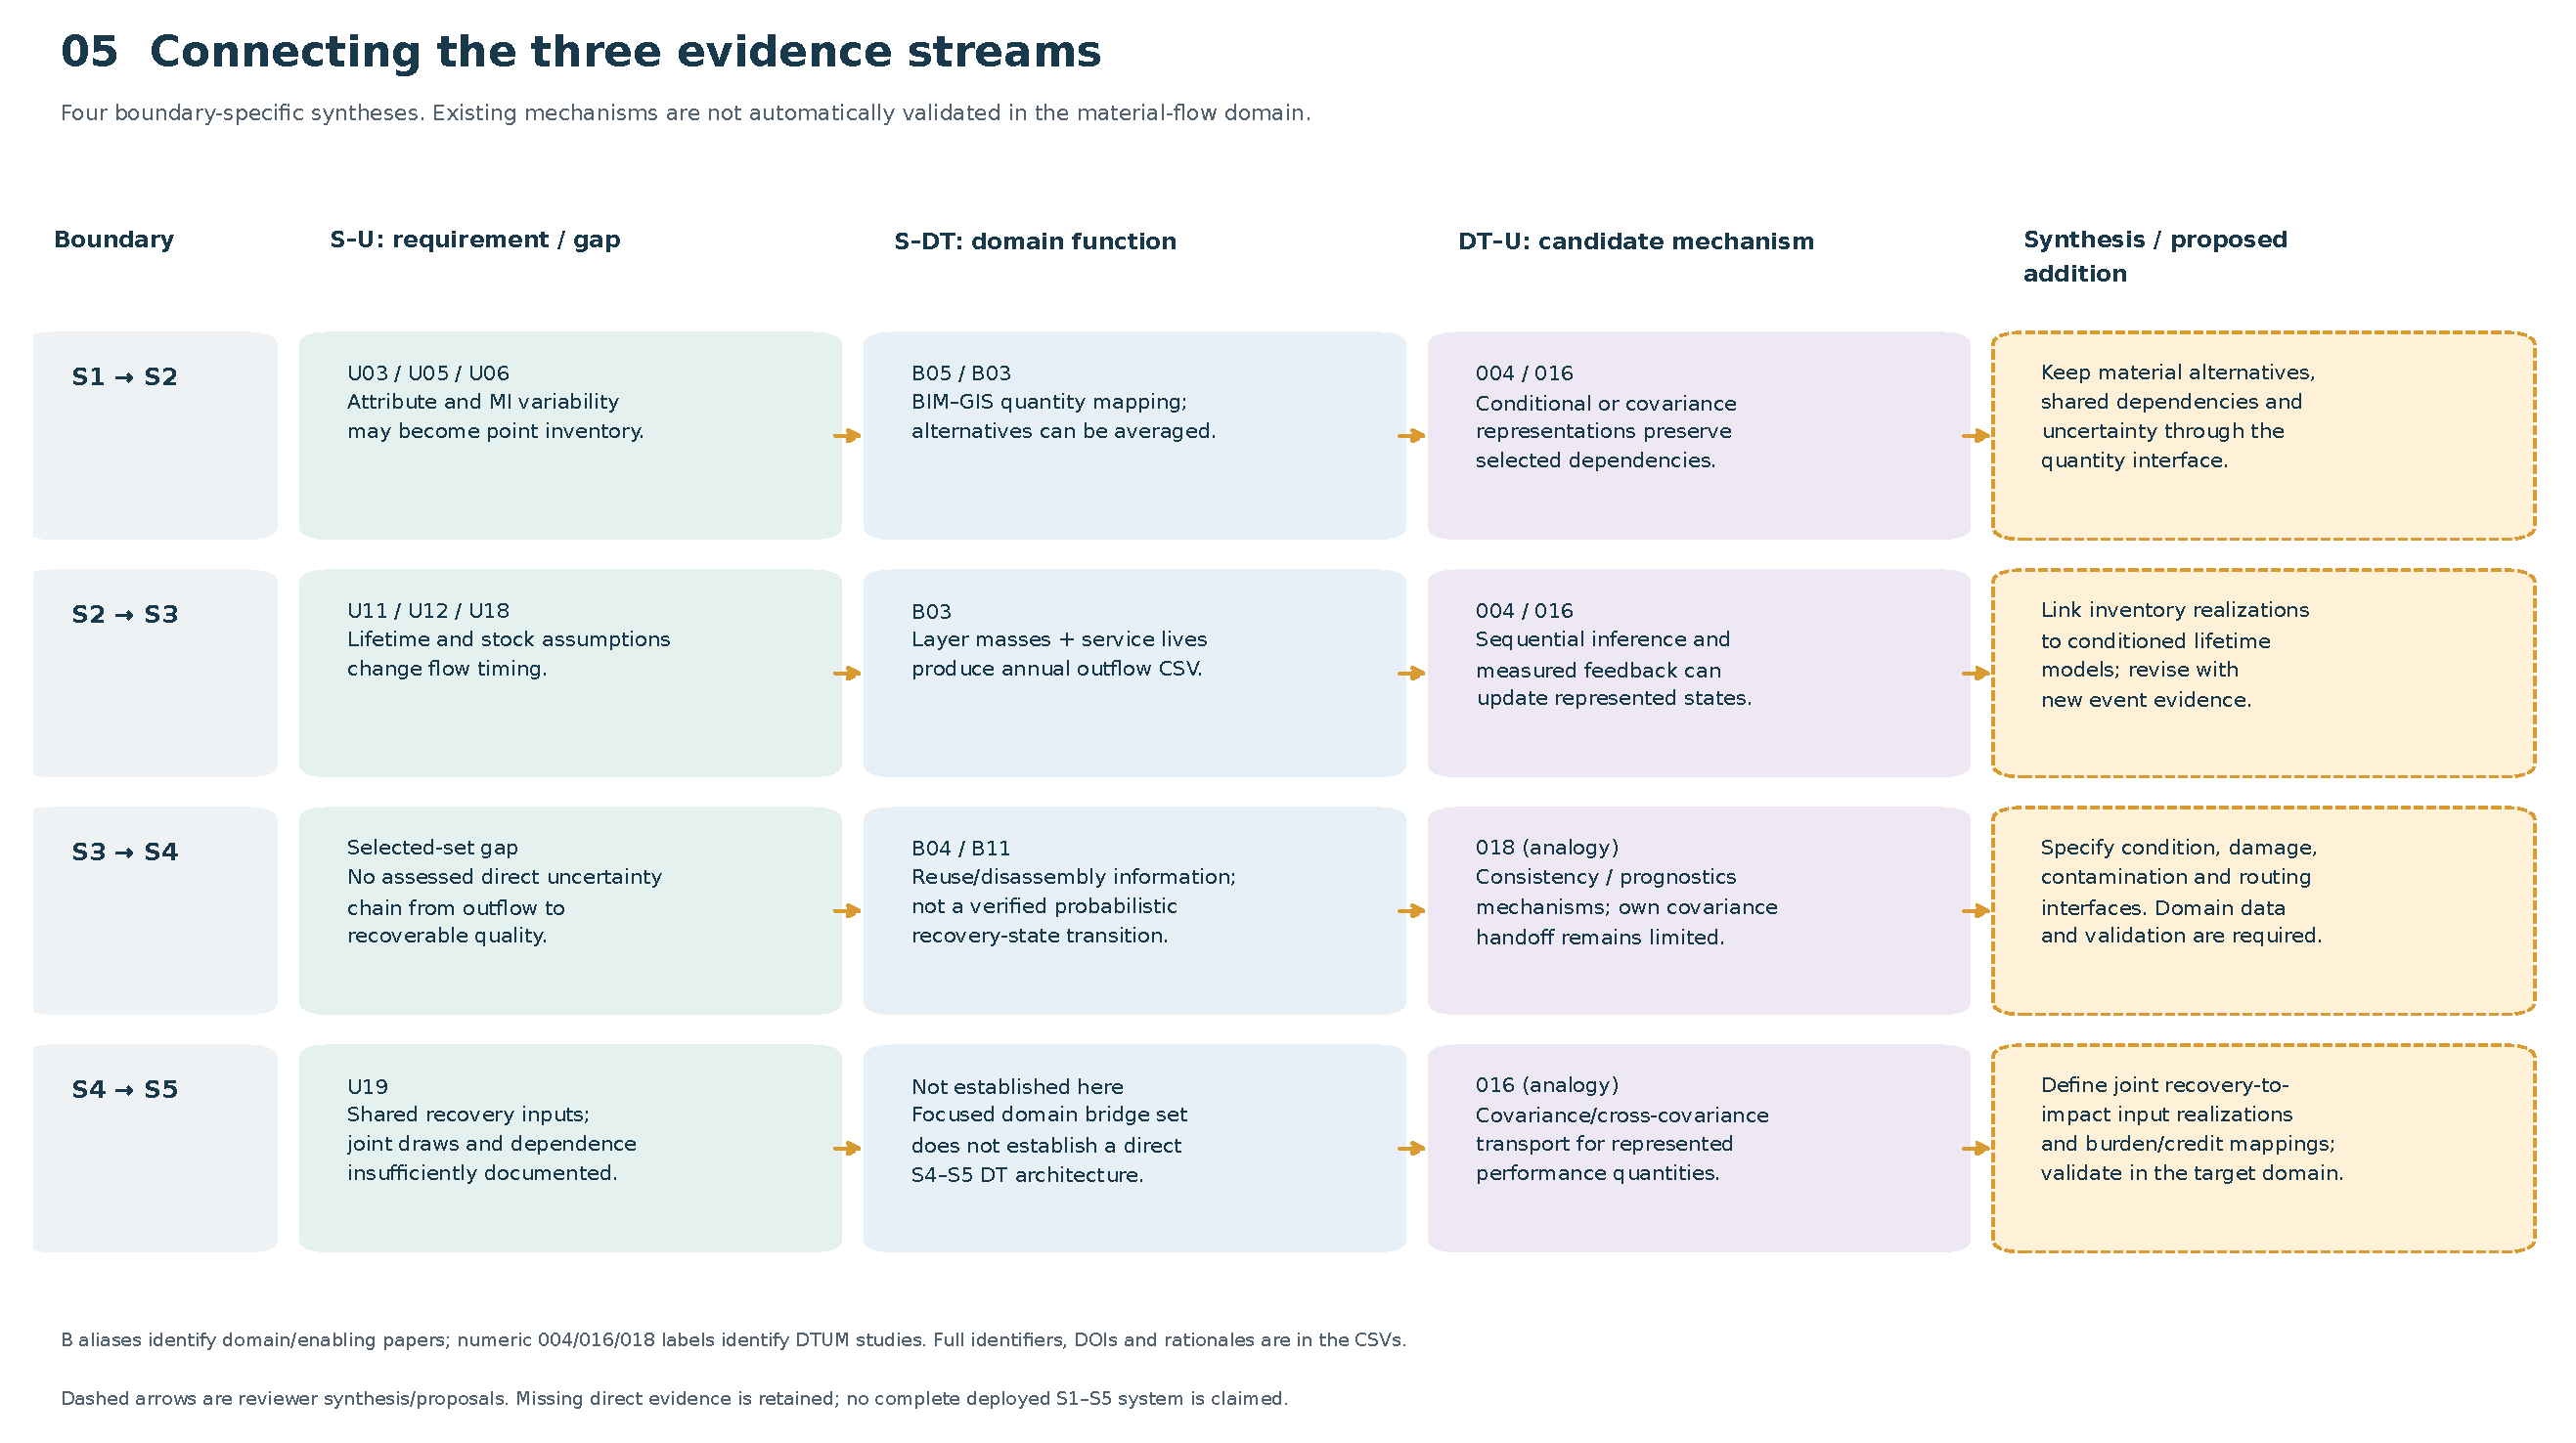
\includegraphics[width=\textwidth]{relational_analysis/conceptual_synthesis/figures/05_evidence_to_architecture.pdf}
\caption{Four boundary-specific paths connecting uncertainty requirements, domain functions and candidate DT uncertainty mechanisms. Dashed arrows and the final column denote reviewer synthesis or proposed gap responses. Generic mechanisms require compatibility assessment and validation before transfer to material-flow applications.}
\label{fig:relational-paths}
\end{figure*}

\begin{figure*}[t]
\centering
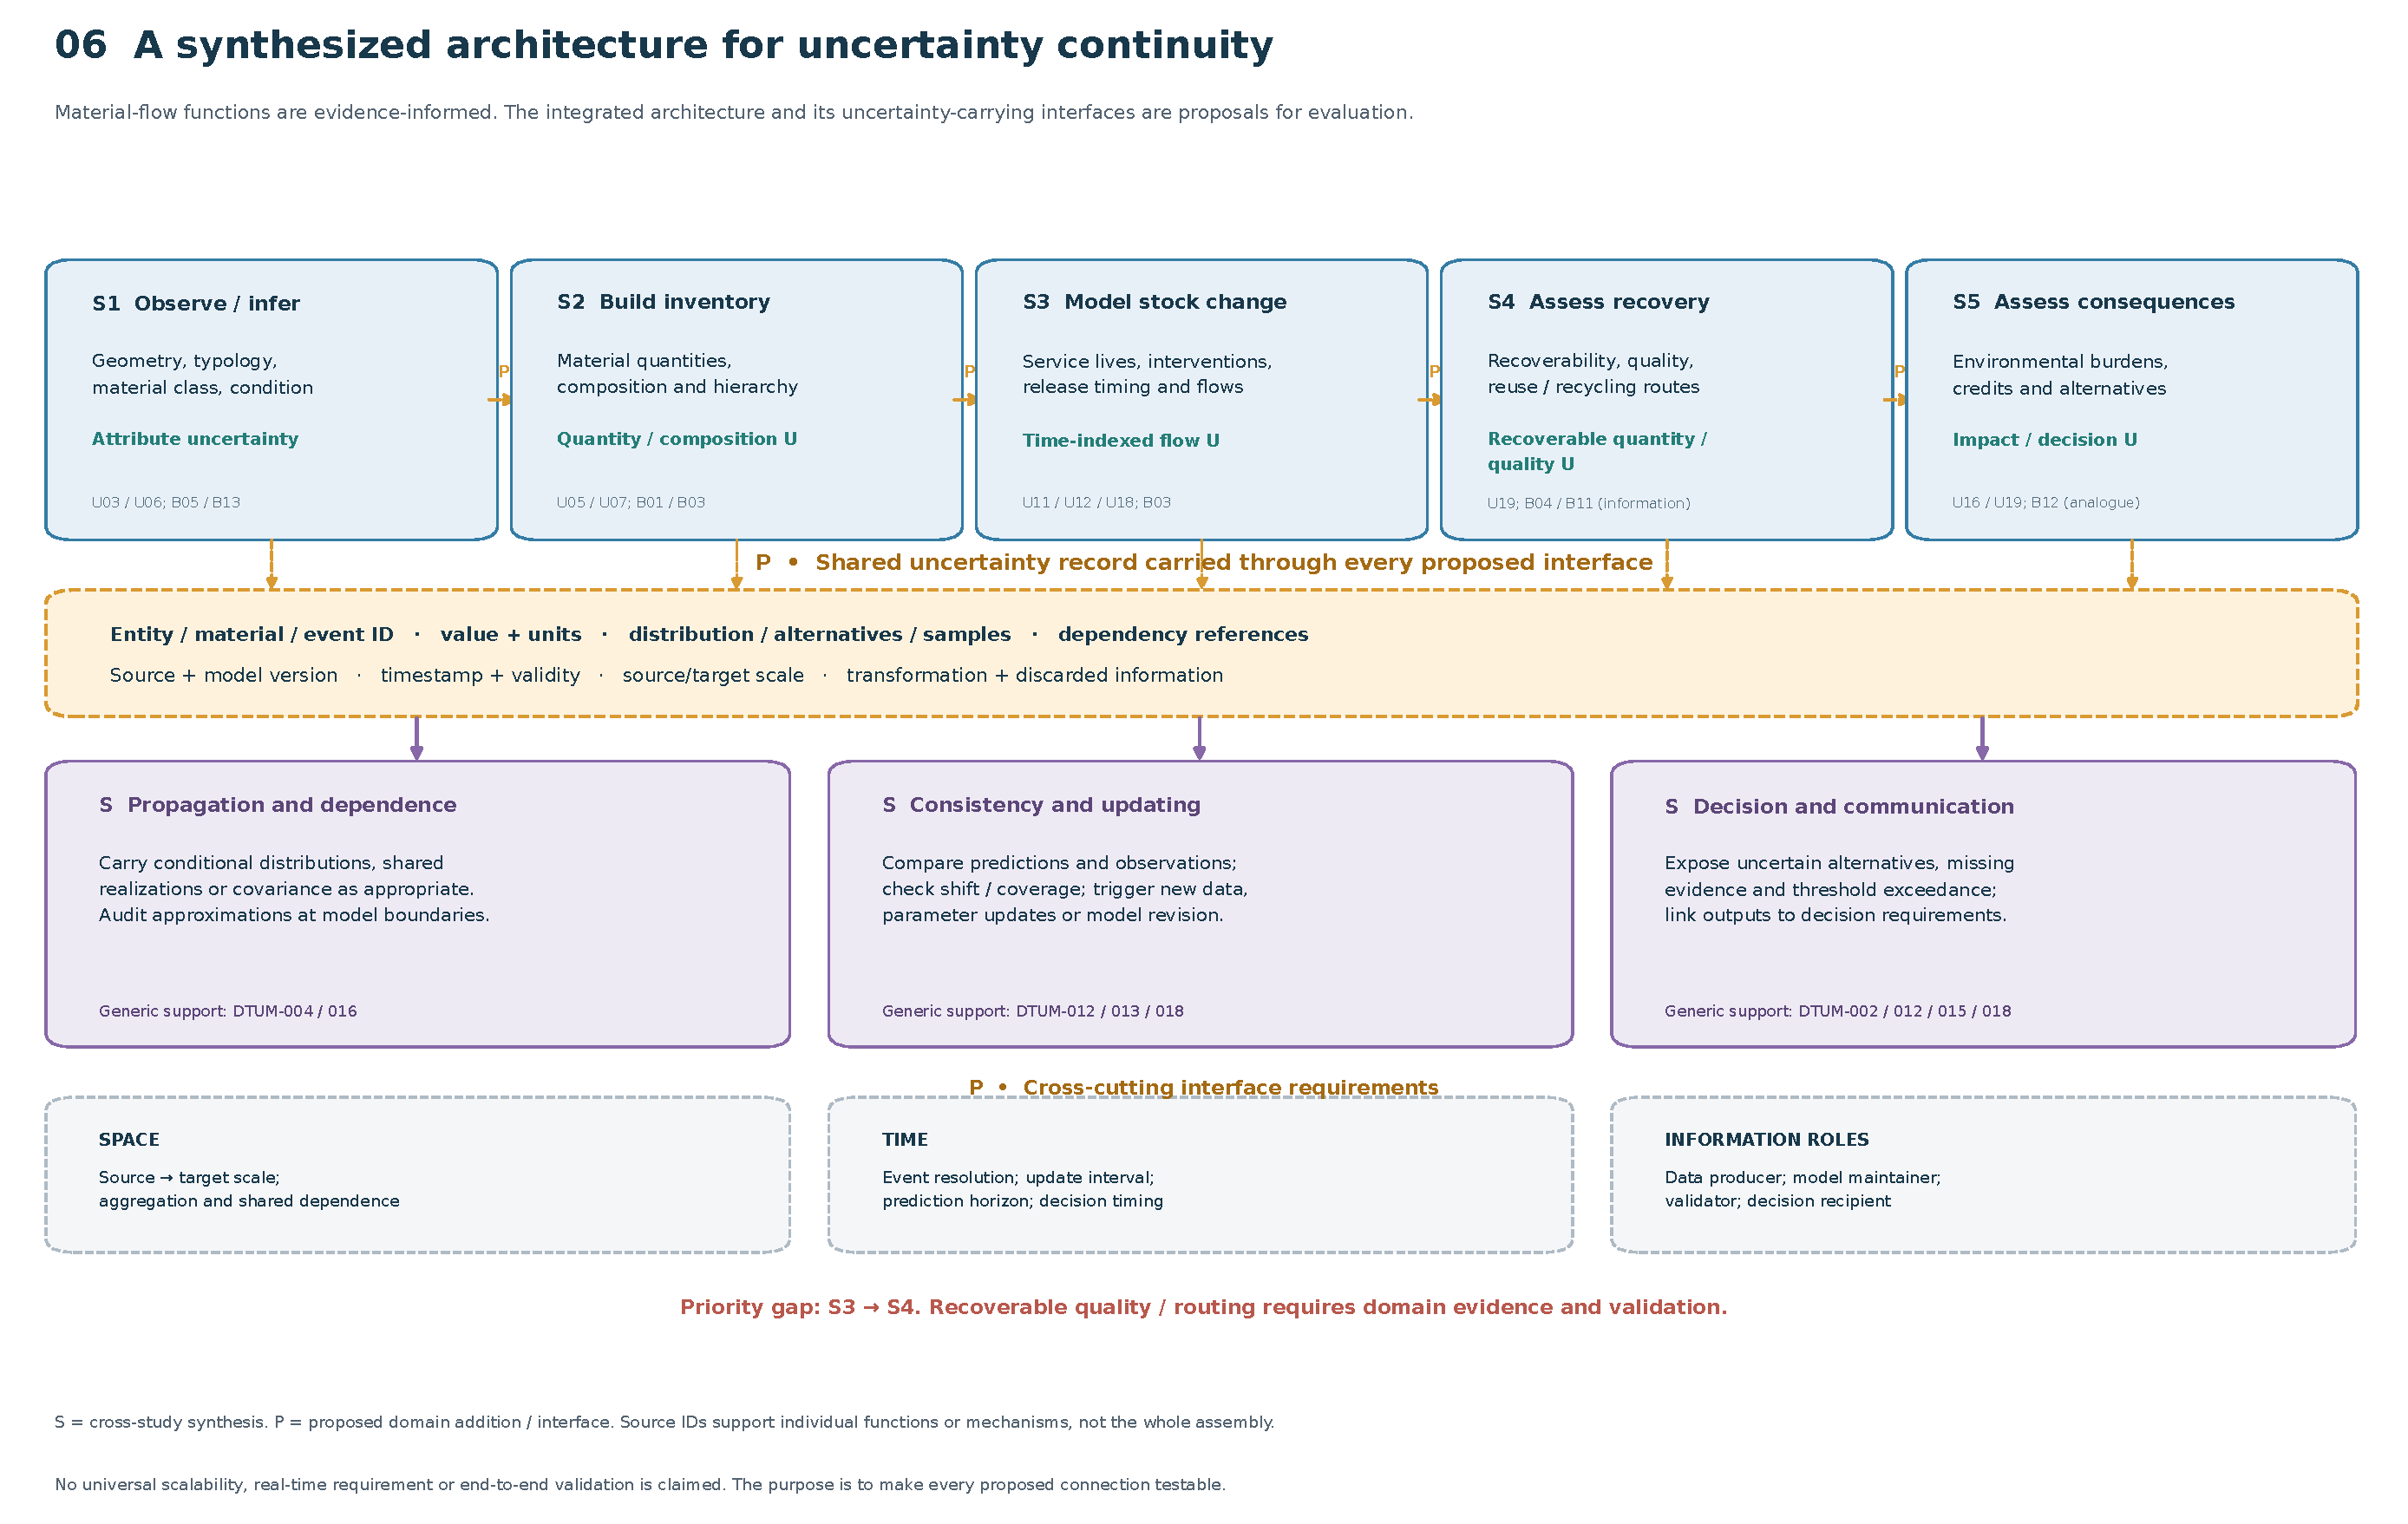
\includegraphics[width=\textwidth]{relational_analysis/conceptual_synthesis/figures/06_synthesized_architecture.pdf}
\caption{Evidence-informed architecture proposed for uncertainty continuity in circular built-environment material flows. Source identifiers support individual functions and mechanisms, not the assembled system. S denotes cross-study synthesis and P a proposed interface or domain addition. Space, timing and information roles constrain the interfaces; neither universal scalability nor end-to-end validation is claimed.}
\label{fig:relational-architecture}
\end{figure*}
